% LaTeX template for URSI Radio Science Letters (RSL)
%
% Use pdflatex or latex + dvips + ps2pdf to produce a PDF.
%
% 15 June 2021, Henrik Wallen <henrik.wallen@aalto.fi>

%
% Submissions to RSL must use the default class option [manuscript].
% At other stages the [preprint] option can be handy.
%
\documentclass[preprint]{rsl}
%\documentclass{rsl}

%
% DO NOT add any packages or define custom macros.
%

% Title and author(s)
%
% Use explicit line-breaks \\ if needed and note that the affiliations are
% at the end of the manuscript.
%
\title{On-Body Path Loss Modeling at D-Band Frequencies}
\author{Brecht De Beelde,	% 1st author
Reza~Aminzadeh,	% 2nd author
Emmeric~Tanghe,	% 3rd author
David~Plets,		% 4th author
Wout~Joseph		% 5th author
}

\begin{document}

\maketitle

%
% Manuscript contents begins.
%

\begin{abstract}

This letter presents an on-body path loss model

\end{abstract}

\section{Introduction\label{sect:intro}}

Link to paper by Reza \cite{Aminzadeh2021_tap}. 

Section~\ref{sect:method} provides the measurement setup and scenarios. 
Section~\ref{sect:results} provide the measurement results and path loss model, and Section~\ref{sect:conclusion} concludes this letter.

\section{Methodology \label{sect:method}}

A vector network analyzer (VNA) with frequency convertors is used to perform D-band channel measurements for antenna separations up to 20~cm, with a skin phantom positioned between the antennas. 
This measurement setup is presented in Fig.~\ref{fig:sounder_setup}.
\begin{figure}[tb]
\begin{center}
	\includegraphics[width=0.45\textwidth]{figures/measurement_setup}
\caption{Picture of the measurement setup with vector network analyzer-based channel sounder.}
\label{fig:sounder_setup}
\end{center}
\end{figure}

\subsection{Channel sounder}

The VNA generates a radio frequency (RF) source input from $9.167$ to $14.167$~GHz that is multiplied by a factor 12 via frequency multiplication using an external frequency up-converter, which results in an RF output in the frequency range 110 to 170~GHz. 
A harmonic mixer with multiplication factor 10 and a local oscillator (LO) input in frequency range $10.972$ to $16.9782$~GHz, is used for down-conversion, and generates a reference signal for the VNA. 
A standard gain pyramidal horn antenna with a gain increasing from 22.2~dBi for 110~GHz  to 23.3~dBi for 170~GHz is connected to the frequency converter's WR-6 waveguide and transmits the D-band signal.
At the receiver side, an identical antenna captures the received signal, which is down-converted using the harmonic mixer of the frequency down-converter that uses the same LO input. 
The down-converted signal is sent to the measurement port of the VNA. 
The VNA measures the phase and amplitude difference between the reference signal at port 1 and the measured signal at port 2.
The antennas have a H-plane half power beam width (HPBW) ranging from 13.2$^{\circ}$ at 110~GHz to 12$^{\circ}$ at 170~GHz and an E-plane HPBW ranging from 12$^{\circ}$ at 110~GHz to 8.8$^{\circ}$ at 170~GHz. 
The Fraunhofer far-field distance $d_F$ of these antennas, calculated via (\ref{eq:Fraunhofer}), equals 0.55~m at 170~GHz as $D$ is equal to 0.022~m and the wavelength $\lambda$ is 0.00176 m.
\begin{equation}
\label{eq:Fraunhofer}
d_F = \frac{2 D^2}{\lambda}
\end{equation}

We perform a frequency sweep with 3001 frequency points and a frequency step size of 20~MHz. 
The intermediate frequency (IF) measurement bandwidth (BW) of the VNA is set to 100~Hz. 
The output power is set to 16 dBm.
A normalized forward calibration is performed before all measurements, with the converters' WR-6 waveguides as the reference plane of the calibration. 
No averaging is performed on the VNA, but each measurement is performed three times.
The VNA's sweep time is 45~s during which the channel is assumed to be static, as no people were moving during the measurements. 

The IF BW and transmit power settings result in a dynamic range of the sounder of 95~dB.
Due to the high bandwidth, a high temporal resolution $\Delta\tau$ of $0.0167$~ns is obtained.
The maximum resolvable time delay of 50~ns corresponds to a path length of 15~m.
The validation of the channel sounder is presented in previous work \cite{DeBeelde2021}. 

\subsection{Measurement scenarios}

Reference measurement are performed with an antenna separation of 1~m, i.e., the antennas are in the far field. 
Absorbers are placed to limit the environmental influence.
The reference measurements are used to evaluate antenna gains, cable losses, and conversion losses over the full band. 

For the on-body PL measurements, the antenna separation ranges from 1~cm to 19~cm, by moving the RX antenna away from the TX antenna in steps of 3~cm.
In between the antennas, a skin phantom is placed. 
The antennas are placed at different heights above the skin phantom of respectively 1~mm, 3~mm, and 6~mm. 
Measurements are performed with both horizontal (HH) and vertical (VV) co-polarized antennas.

\subsection{Skin phantom}

Information on the skin phantom comes here.

\subsection{Data processing}

From the measured transfer function $H(f)$, PL is obtained via (\ref{eq:PL}), with $N$ the number of frequency sweeps, $G_a(f)$ the frequency-dependent antenna gain and $C(f)$ a correction term based on reference measurements that are performed in the center of the lab, without nearby reflectors \cite{DeBeelde2021}.
\begin{equation}
\label{eq:PL}
\text{PL}_{\text{dB}}(f)= -10 \text{log}_{10} \left( \frac{1}{N} \sum_{i=1}^N | H_i(f) |^2 \right) + 2 G_a(f) + C(f)
\end{equation}
After applying the Hann window $\mathcal{W}$, the inverse discrete Fourier transformation (IDFT) of the transfer function $H(f)$ results in the channel impulse response (CIR) from which the averaged power delay profile (PDP) is found via (\ref{eq:PDP}).
\begin{equation}
\text{PDP}(k\Delta\tau) = \frac{1}{N} \sum_{i=1}^N | \text{IDFT}(\mathcal{W}(f) \cdot H_i(f)) |^2
\label{eq:PDP}
\end{equation}
The temporal resolution of the PDP $\Delta\tau$ is XX~ns, and the maximum resolvable time domain is XX~ns.
From the PDP, the root-mean-squared (RMS) delay spread is calculated via (\ref{eq:DS}), with \dots
\begin{equation}
\text{PDP}(k\Delta\tau) = \dots
\label{eq:DS}
\end{equation}
Wideband on-body PL is obtained by comparing the power of the first peak of the PDP to the power of the first peak of the reference measurements, i.e., without the skin phantom placed close to the antennas. 
This is represented in (\ref{eq:WB-PL}), with \dots
\begin{equation}
\text{PL}_\text{dB} = \dots
\label{eq:WB-PL}
\end{equation}

Measured PL as a function of frequency, obtained via (\ref{eq:PL}), is fitted to the alpha-beta-gamma (ABG) model from (\ref{eq:ABG}), with $d$ the distance in m, d$_0$ the reference distance, $f$ the frequency in GHz, and f$_0$ the reference frequency.  
In this work, a reference distance d$_0$ of 1~cm and a reference frequency f$_0$ of 1~GHz is selected.
The model parameter $\alpha$ is the floating intercept in dB, i.e., the PL for distance d$_0$ at frequency f$_0$, $\beta$ is the dimensionless PL exponent, $\gamma$ is the dependence of PL on frequency, and $\chi_{\sigma}$ is the shadow fading term in dB \cite{Salous2020}. 
\begin{equation}
  \text{PL}_{\text{ABG}}(d,f) = \alpha + 10 \beta \log_{10}\left(\frac{d}{\text{d}_0}\right) + 10 \gamma \log_{10}\left(\frac{f}{ \text{f}_0}\right) + \chi_{\sigma}
  \label{eq:ABG}
\end{equation}

Wideband PL, obtained via (\ref{eq:WB-PL}), is fitted to the floating-intercept (FI) PL model from (\ref{eq:FI}), with $d$ the distance in m, d$_0$ the reference distance of 1~cm and PL exponent n. 
The shadow fading term $\chi_\sigma$ in dB is again based on a zero-mean normal distribution with standard deviation $\sigma$. 
\begin{equation}
  \text{PL}_{\text{FI}}(d) = \text{PL}_0 + 10 \text{n} \log_{10} (d/\text{d}_0) + \chi_\sigma
  \label{eq:FI}
\end{equation}

\section{Results\label{sect:results}}

Figure~\ref{fig:PL_vs_freq} visualized measured PL as a function of frequency for two polarizations and two distances, with an antenna height of 1~mm.
\begin{figure}[tb]
\begin{center}
	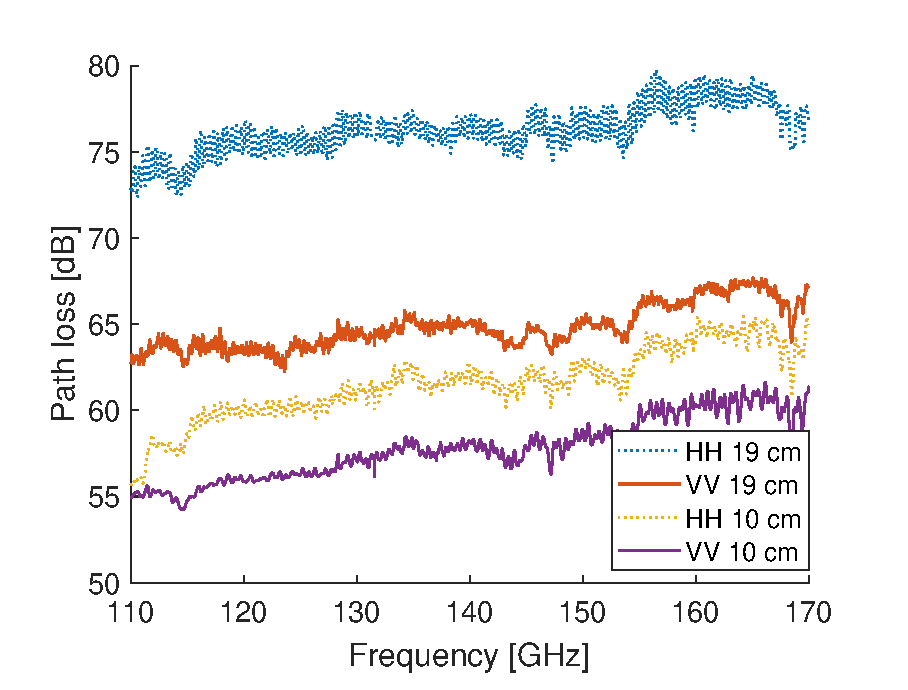
\includegraphics[width=0.45\textwidth]{figures/PL_vs_freq}
\caption{Measured path loss as a function of frequency for antenna height 1~mm above the skin phantom.}
\label{fig:PL_vs_freq}
\end{center}
\end{figure}

Fitting measurement data to the ABG model results in the fitted parameters listed in Table~\ref{table:ABG}. 
\begin{table}
  \caption{Fitted parameters of the ABG model for different polarizations (P) and antenna heights (H) above the skin phantom.}
  \label{table:ABG}
  \begin{center}
    \begin{tabular}{cc|cccc}
      P & H [mm] & $\alpha$ & $\beta$ & $\gamma$ & RMSE \\
      \hline
      VV & 1 \\
      VV & 2\\
      VV & 3\\
      HH & 1\\
      HH & 2\\
      HH & 3\\
    \end{tabular}
  \end{center}
\end{table}
Table~\ref{table:FI} lists the fitted parameters of the FI PL model from (\ref{eq:FI}). \emph{Fit for different polarizations/antenna heights or is there another approach?}
\begin{table}
  \caption{Fitted parameters of the FI model for different polarizations (P) and antenna heights (H) above the skin phantom.}
  \label{table:FI}
  \begin{center}
    \begin{tabular}{cc|cccc}
      P & H [mm] & PL$_0$ & n& RMSE \\
      \hline
      VV & 1 \\
      VV & 2\\
      VV & 3\\
      HH & 1\\
      HH & 2\\
      HH & 3\\
    \end{tabular}
  \end{center}
\end{table}

Figure~\ref{fig:PDP} shows the PDP for some select measurement scenarios. 
It is clear that round-trip reflections, i.e., reflections on the TX and RX antennas, are present. 
These reflections cause a pulse to spread in time, which reflects on the RMS delay spread values that range from XX~ns for YY to ZZ~ns for WW.
\begin{figure}[tb]
\begin{center}
%	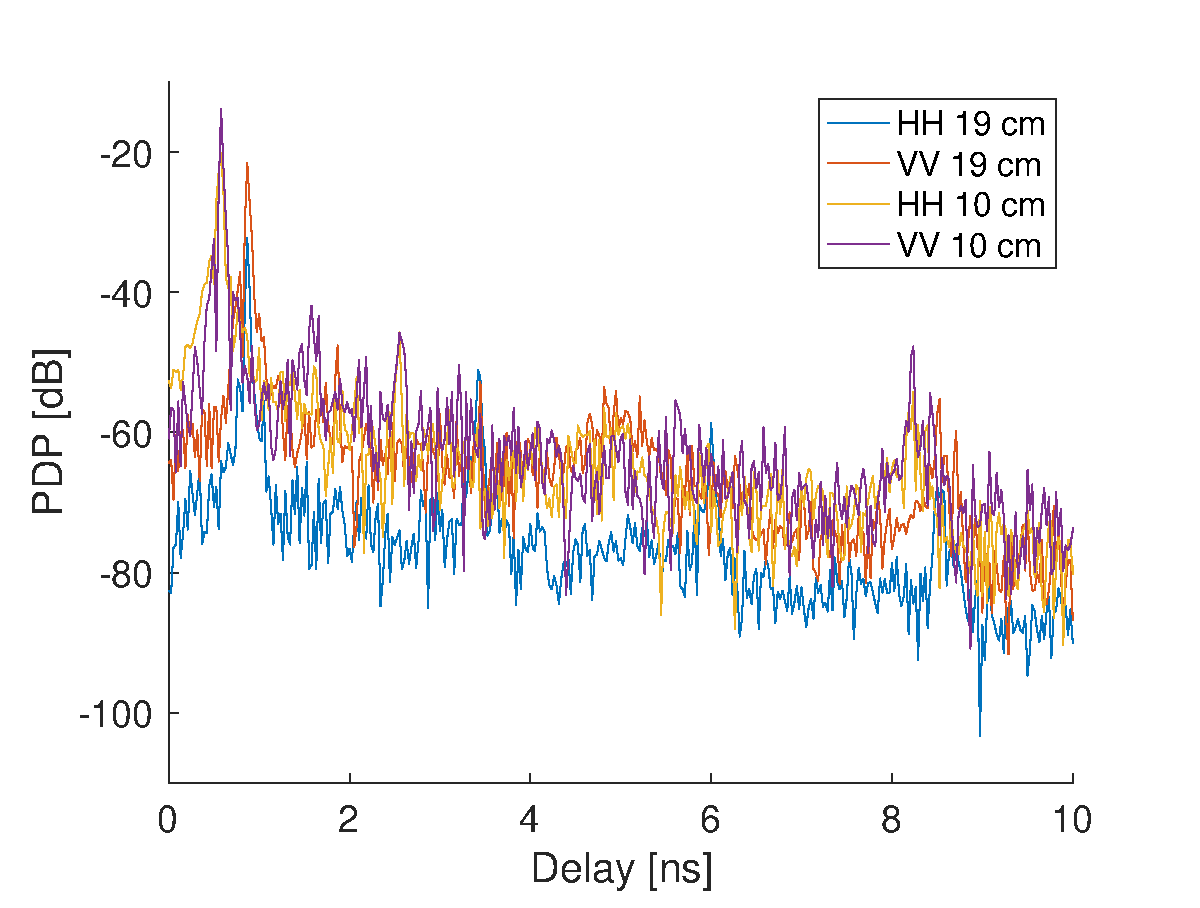
\includegraphics[width=0.45\textwidth]{figures/PDP}
\caption{Measured power delay profile (PDP) for antenna heights 1~mm and 3~mm above the skin phantom.}
\label{fig:PDP}
\end{center}
\end{figure}
The reflections on the skin phantom cannot be resolved in the PDP, as the direct and reflected path lengths differ by less than XX~cm.

\section{Conclusions\label{sect:conclusion}}

In this letter, \dots

Future work includes the validation of the PL models on a real human body, and taking into account antenna mismatch, e.g., cause by wrist rotation.

\section{Acknowledgment}

This work was executed within the imec AAA D-band channel modeling research project (D-BARC) and EOS project multi-service wireless network (MUSE-WINET). 
D-BARC received support from Flanders Innovation \& Entrepreneurship.

\vspace{3pt}

\suppressfloats
\bibliographystyle{IEEEtran}
\bibliography{RSL_140GHz_body}
\suppressfloats

\vspace{7pt}

%
% Note that the authors' affiliations and contact information should be
% here, after the references.
%
\noindent\small
B. De Beelde, E. Tanghe, D. Plets and W. Joseph are with Ghent University/IMEC, Department of Information Technology, Ghent, Belgium. 
R. Aminzadeh is with Unitron Group. 
Corresponding author: B. De Beelde. 
E-mail:Brecht.DeBeelde@UGent.be
\end{document}
